\section{Versuchsaufbau}

\subsection{Teil I: Pockels-Effekt}
\begin{figure}[H]
\begin{center}
  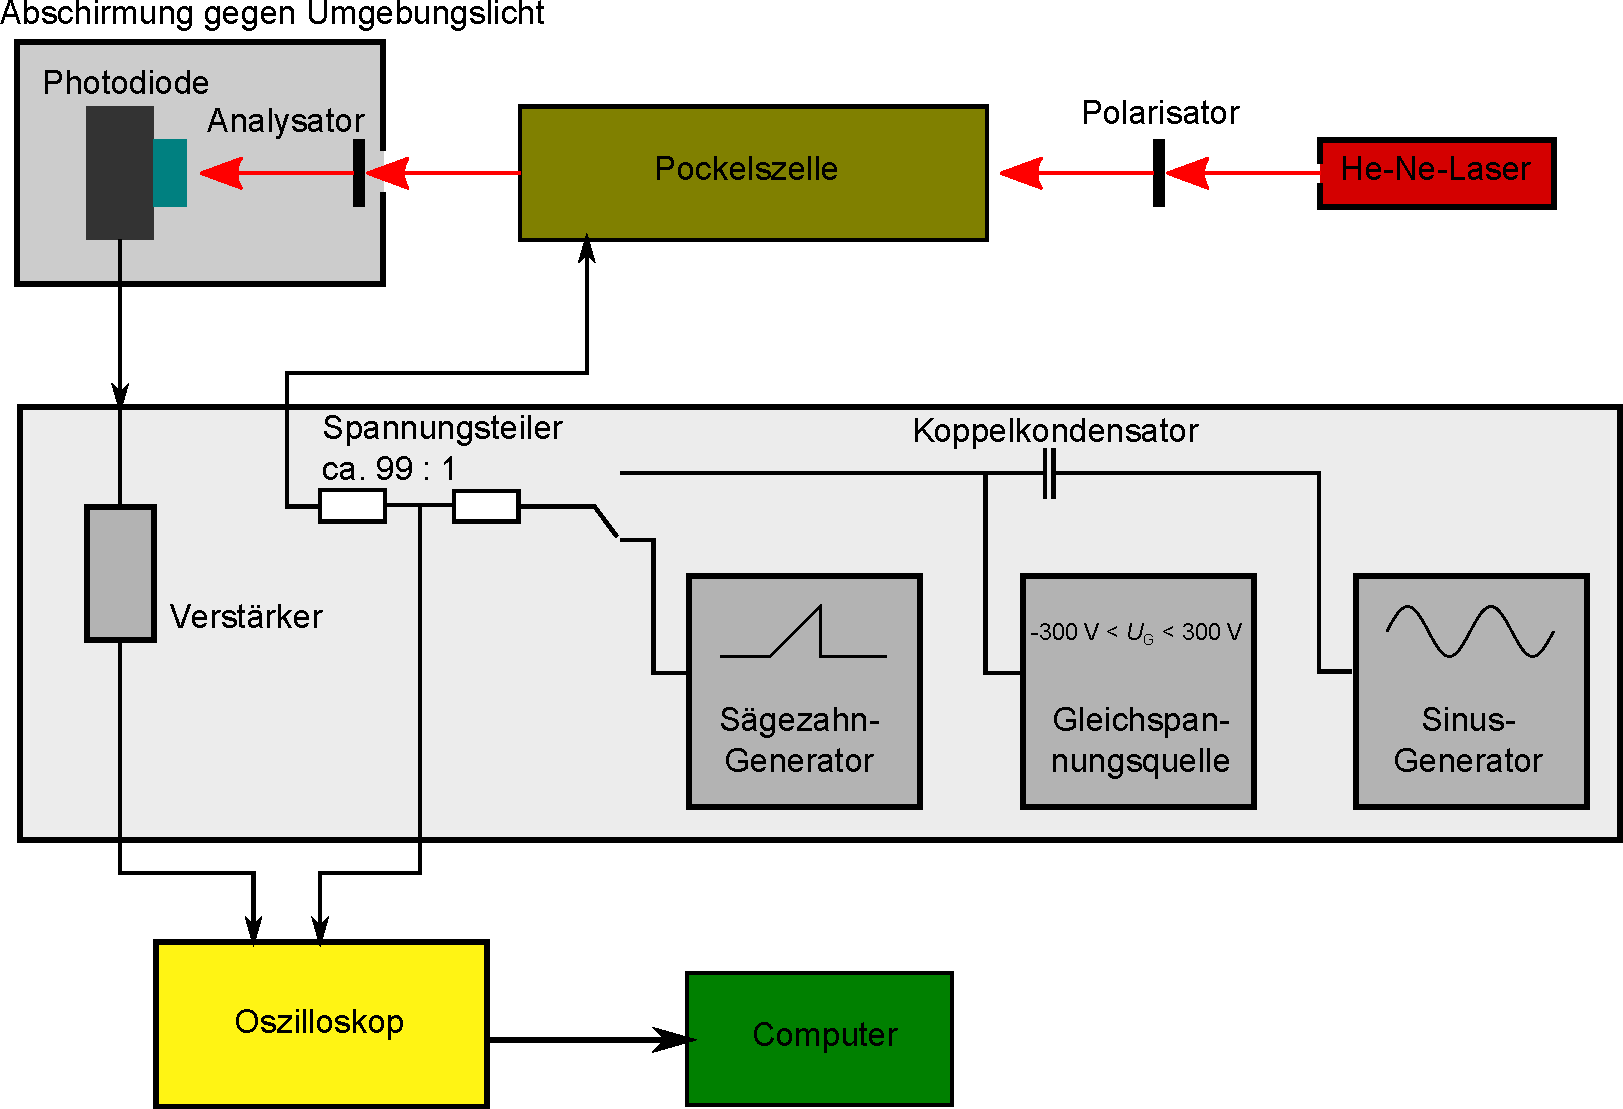
\includegraphics[width=\textwidth]{../img/aufbauPock.pdf}
  \caption{Aufbau zur Messung der spannungsabhängigen Polarisationsdrehung von Licht in der Pockelszelle.}
  \label{img:aufbauPock}
\end{center}
\end{figure}
\autoref{img:aufbauPock} zeigt den Aufbau, mit dem die Messungen an der Pockelszelle durchgeführt werden.
Der Strahl eines Helium-Neon-Lasers wird linear polarisiert und fällt in die Zelle.
Dort liegt eine Spannung an, die an drei Netzteilen eingestellt wird:
Es kann eine Sägezahnspannung mit 500\,V Amplitude angelegt werden oder
eine Gleichspannung zwischen -300\,V und 300\,V,
der eine Sinusspannung mit einstellbarer Frequenz und Amplitude überlagert werden kann.
Über einen Spannungsteiler, der die Spannung auf ungefähr ein Hundertstel ihrer Amplitude reduziert,
kann das Signal an der Pockelszelle auf einem Oszilloskop betrachtet werden.\\
Nach der Zelle fällt das Laserlicht auf einen drehbaren Analysator und anschließend auf eine Photodiode,
deren Signal verstärkt an das Oszilloskop weitergeleitet wird.
Die Photodiode ist gegen Umgebungslicht abgeschirmt.
Mit dem Computer kann des Oszilloskop ausgelesen werden.


\subsection{Teil II: Faraday-Effekt}
